We have implemented the test suite over the \texttt{lnd} framework~\cite{lndDaemon}, 
a complete implementation of the Lightning node written in Go.
We use the command-line interface to access to routing information, 
gather routes and generate requests modified to suit to our measuring algorithm~\ref{sec:methodology}.

We have validated the testing methodology locally over the topology depicted in figure~\ref{fig:local-test-topology}, 
being each node an instance of the \texttt{lnd} daemon.
We create the channel to test, $C_{1,2}$, as follows: 
we command $N_1$ to execute a \texttt{connect} command in the Lightning command line interface 
(lncli) to $N_2$, and then we execute openchannel 
\ed{We dont know if openchannel negotiates or receives information from $N_2$ or not}
and it performs the funding transaction of the channel.

With this configuration, node $N_1$ advertises the funding capacity for the channel.
\ed{We are almost sure that $N_2$ does not advertise anything. Check what is the infomation $N_3$ receives}.

After this, $N_0$ can issue a transaction to $N_3$.
For this, it request a route. \ed{Check if this gathers information from $N_1$, and if so, which information. We think it does not receive information about the current balance, and we do not know which are the things it requests...but then we do not understand why it takes so much time and 
Execute strace for route request...}

If $N_3$ request a route for $N_0$, it does not receive any. However, we can build a route by generating manually information of the $N_2$ to $N_1$ hop, and then for the $N_1$ to $N_0$ hop.
If there is enough balance at $N_2$, then the transaction request is accepted and passed to $N_1$, and the same occurs from $N_1$ to $N_0$. Therefore, it is possible to perform the payment, but 
this way of paying is not provided out-of-the-box by the \texttt{lnd} suite.
\ed{we should know why is this}

We test with different capacities for the channel $C_{A,B}$, and execute the capacity estimation algorithm for path 
$\langle N_0$, $N_1$, $N_2$, $N_G \rangle$, and  path $\langle N_3$, $N_2$, $N_1$, $N_G \rangle$. 
We have checked in all cases that the sum of the measured capacities 
is consistent with the funding capacity (within the error margin of the capacity estimation).

We now test the case when one of the nodes is disconnected, i.e., $N_2$ for $\langle N_0$, $N_1$, $N_2$, $N_3 \rangle$ testing has been powered-off. 
...
Additionally, we show the result when $N_0$ is powered-off.

Test with $\epsilon$ (also for known balance, lower than funding capacity, test balance+$\epsilon$).

understand dust\_limit\_satoshis: 
Test dust\_limit\_satoshis 'is the threshold below which outputs should not be generated for this node's commitment or HTLC transactions (i.e., HTLCs below this amount plus HTLC transaction fees are not enforceable on-chain). This reflects the reality that tiny outputs are not considered standard transactions and will not propagate through the Bitcoin network.'
This may affect the fee, the amount to pay, or both.
So I would say $\epsilon=dust\dots$.
Which is the default value for this?



Other cases are: errors that may occur, how to generate them.
\ed{We don't know if there are behaviours specific to the daemon}

\begin{figure}[h!]
    \centering
    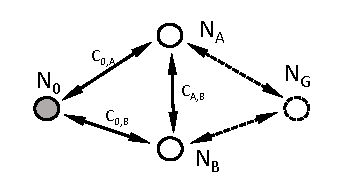
\includegraphics[width=0.99\linewidth]{img/local-test-topology.pdf}
    \caption{Local test topology}
    \label{fig:local-test-topology}
\end{figure}




